\documentclass[14pt]{extbook}
\usepackage{multicol, enumerate, enumitem, hyperref, color, soul, setspace, parskip, fancyhdr} %General Packages
\usepackage{amssymb, amsthm, amsmath, latexsym, units, mathtools} %Math Packages
\everymath{\displaystyle} %All math in Display Style
% Packages with additional options
\usepackage[headsep=0.5cm,headheight=12pt, left=1 in,right= 1 in,top= 1 in,bottom= 1 in]{geometry}
\usepackage[usenames,dvipsnames]{xcolor}
\usepackage{dashrule}  % Package to use the command below to create lines between items
\newcommand{\litem}[1]{\item#1\hspace*{-1cm}\rule{\textwidth}{0.4pt}}
\pagestyle{fancy}
\lhead{Progress Quiz 7}
\chead{}
\rhead{Version ALL}
\lfoot{3510-5252}
\cfoot{}
\rfoot{Summer C 2021}
\begin{document}

\begin{enumerate}
\litem{
Construct the lowest-degree polynomial given the zeros below. Then, choose the intervals that contain the coefficients of the polynomial in the form $ax^3+bx^2+cx+d$.\[ \frac{-4}{5}, \frac{-1}{2}, \text{ and } \frac{2}{5} \]\begin{enumerate}[label=\Alph*.]
\item \( a \in [47, 51], b \in [44, 46], c \in [-10, -4], \text{ and } d \in [5, 10] \)
\item \( a \in [47, 51], b \in [-86, -79], c \in [41, 48], \text{ and } d \in [-11, -2] \)
\item \( a \in [47, 51], b \in [-50, -44], c \in [-10, -4], \text{ and } d \in [5, 10] \)
\item \( a \in [47, 51], b \in [44, 46], c \in [-10, -4], \text{ and } d \in [-11, -2] \)
\item \( a \in [47, 51], b \in [-35, -28], c \in [-16, -10], \text{ and } d \in [5, 10] \)

\end{enumerate} }
\litem{
Describe the zero behavior of the zero $x = 4$ of the polynomial below.\[ f(x) = -5(x + 4)^{6}(x - 4)^{7}(x + 5)^{3}(x - 5)^{6} \]\begin{enumerate}[label=\Alph*.]
\begin{multicols}{2}\item 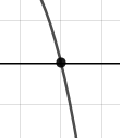
\includegraphics[width = 0.3\textwidth]{../Figures/polyZeroBehaviorCopyAA.png}\item 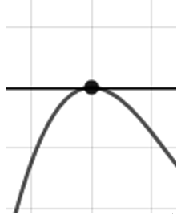
\includegraphics[width = 0.3\textwidth]{../Figures/polyZeroBehaviorCopyBA.png}\item 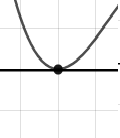
\includegraphics[width = 0.3\textwidth]{../Figures/polyZeroBehaviorCopyCA.png}\item 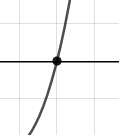
\includegraphics[width = 0.3\textwidth]{../Figures/polyZeroBehaviorCopyDA.png}\end{multicols}\item None of the above.
\end{enumerate} }
\litem{
Which of the following equations \textit{could} be of the graph presented below?
\begin{center}
    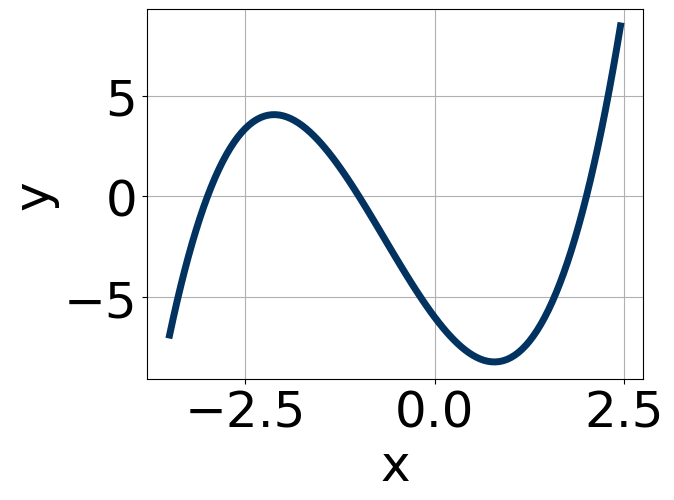
\includegraphics[width=0.5\textwidth]{../Figures/polyGraphToFunctionCopyA.png}
\end{center}
\begin{enumerate}[label=\Alph*.]
\item \( 17(x - 2)^{8} (x + 1)^{9} (x + 3)^{11} \)
\item \( -7(x - 2)^{4} (x + 1)^{7} (x + 3)^{11} \)
\item \( 15(x - 2)^{7} (x + 1)^{5} (x + 3)^{7} \)
\item \( -2(x - 2)^{11} (x + 1)^{9} (x + 3)^{9} \)
\item \( 7(x - 2)^{10} (x + 1)^{8} (x + 3)^{11} \)

\end{enumerate} }
\litem{
Construct the lowest-degree polynomial given the zeros below. Then, choose the intervals that contain the coefficients of the polynomial in the form $x^3+bx^2+cx+d$.\[ -4 - 2 i \text{ and } -1 \]\begin{enumerate}[label=\Alph*.]
\item \( b \in [0, 4], c \in [4.37, 5.42], \text{ and } d \in [2.7, 4.8] \)
\item \( b \in [6, 11], c \in [27.08, 28.41], \text{ and } d \in [14.4, 20.2] \)
\item \( b \in [-9, -7], c \in [27.08, 28.41], \text{ and } d \in [-20.3, -18.9] \)
\item \( b \in [0, 4], c \in [0.79, 4.62], \text{ and } d \in [-0.4, 3.2] \)
\item \( \text{None of the above.} \)

\end{enumerate} }
\litem{
Which of the following equations \textit{could} be of the graph presented below?
\begin{center}
    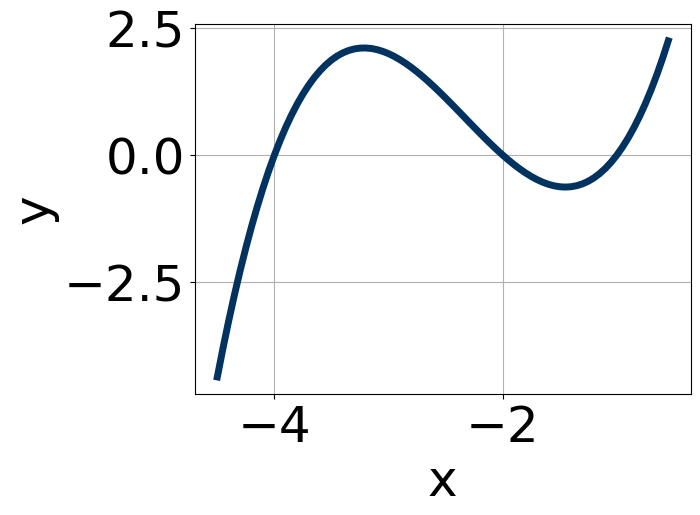
\includegraphics[width=0.5\textwidth]{../Figures/polyGraphToFunctionA.png}
\end{center}
\begin{enumerate}[label=\Alph*.]
\item \( -7(x + 1)^{5} (x + 2)^{9} (x + 4)^{9} \)
\item \( 10(x + 1)^{10} (x + 2)^{5} (x + 4)^{7} \)
\item \( 9(x + 1)^{9} (x + 2)^{7} (x + 4)^{11} \)
\item \( -2(x + 1)^{10} (x + 2)^{5} (x + 4)^{5} \)
\item \( 20(x + 1)^{10} (x + 2)^{8} (x + 4)^{9} \)

\end{enumerate} }
\litem{
Describe the zero behavior of the zero $x = 3$ of the polynomial below.\[ f(x) = 6(x + 5)^{4}(x - 5)^{2}(x + 3)^{13}(x - 3)^{8} \]\begin{enumerate}[label=\Alph*.]
\begin{multicols}{2}\item 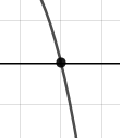
\includegraphics[width = 0.3\textwidth]{../Figures/polyZeroBehaviorAA.png}\item 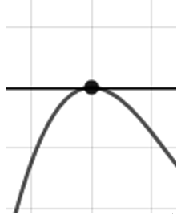
\includegraphics[width = 0.3\textwidth]{../Figures/polyZeroBehaviorBA.png}\item 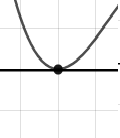
\includegraphics[width = 0.3\textwidth]{../Figures/polyZeroBehaviorCA.png}\item 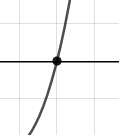
\includegraphics[width = 0.3\textwidth]{../Figures/polyZeroBehaviorDA.png}\end{multicols}\item None of the above.
\end{enumerate} }
\litem{
Describe the end behavior of the polynomial below.\[ f(x) = -9(x - 5)^{3}(x + 5)^{8}(x - 6)^{4}(x + 6)^{6} \]\begin{enumerate}[label=\Alph*.]
\begin{multicols}{2}\item 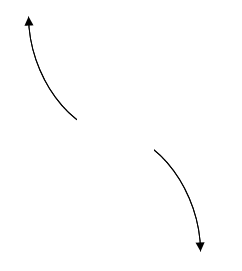
\includegraphics[width = 0.3\textwidth]{../Figures/polyEndBehaviorAA.png}\item 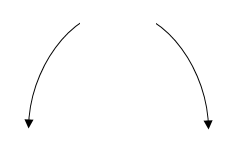
\includegraphics[width = 0.3\textwidth]{../Figures/polyEndBehaviorBA.png}\item 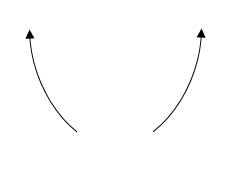
\includegraphics[width = 0.3\textwidth]{../Figures/polyEndBehaviorCA.png}\item 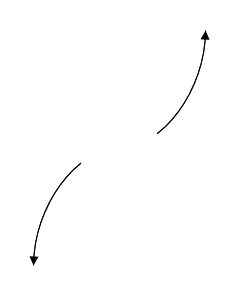
\includegraphics[width = 0.3\textwidth]{../Figures/polyEndBehaviorDA.png}\end{multicols}\item None of the above.
\end{enumerate} }
\litem{
Describe the end behavior of the polynomial below.\[ f(x) = 2(x + 2)^{2}(x - 2)^{7}(x + 8)^{4}(x - 8)^{4} \]\begin{enumerate}[label=\Alph*.]
\begin{multicols}{2}\item 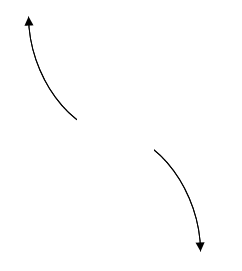
\includegraphics[width = 0.3\textwidth]{../Figures/polyEndBehaviorCopyAA.png}\item 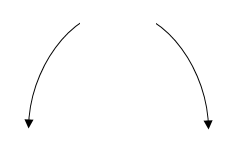
\includegraphics[width = 0.3\textwidth]{../Figures/polyEndBehaviorCopyBA.png}\item 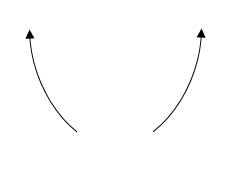
\includegraphics[width = 0.3\textwidth]{../Figures/polyEndBehaviorCopyCA.png}\item 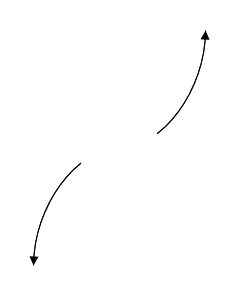
\includegraphics[width = 0.3\textwidth]{../Figures/polyEndBehaviorCopyDA.png}\end{multicols}\item None of the above.
\end{enumerate} }
\litem{
Construct the lowest-degree polynomial given the zeros below. Then, choose the intervals that contain the coefficients of the polynomial in the form $ax^3+bx^2+cx+d$.\[ \frac{4}{3}, \frac{7}{5}, \text{ and } \frac{-1}{3} \]\begin{enumerate}[label=\Alph*.]
\item \( a \in [44, 48], b \in [-108, -105], c \in [40, 50], \text{ and } d \in [-28, -27] \)
\item \( a \in [44, 48], b \in [9, 14], c \in [-86, -82], \text{ and } d \in [-28, -27] \)
\item \( a \in [44, 48], b \in [127, 141], c \in [121, 128], \text{ and } d \in [25, 34] \)
\item \( a \in [44, 48], b \in [-108, -105], c \in [40, 50], \text{ and } d \in [25, 34] \)
\item \( a \in [44, 48], b \in [107, 110], c \in [40, 50], \text{ and } d \in [-28, -27] \)

\end{enumerate} }
\litem{
Construct the lowest-degree polynomial given the zeros below. Then, choose the intervals that contain the coefficients of the polynomial in the form $x^3+bx^2+cx+d$.\[ -5 - 3 i \text{ and } 1 \]\begin{enumerate}[label=\Alph*.]
\item \( b \in [4, 14], c \in [23.5, 25.2], \text{ and } d \in [-34.6, -33] \)
\item \( b \in [-5, 6], c \in [3.8, 6.7], \text{ and } d \in [-6.8, -4] \)
\item \( b \in [-10, -2], c \in [23.5, 25.2], \text{ and } d \in [33.9, 36.6] \)
\item \( b \in [-5, 6], c \in [-1.7, 3.3], \text{ and } d \in [-3.6, -0.7] \)
\item \( \text{None of the above.} \)

\end{enumerate} }
\litem{
Construct the lowest-degree polynomial given the zeros below. Then, choose the intervals that contain the coefficients of the polynomial in the form $ax^3+bx^2+cx+d$.\[ \frac{5}{3}, \frac{-1}{4}, \text{ and } \frac{-5}{2} \]\begin{enumerate}[label=\Alph*.]
\item \( a \in [23, 25], b \in [-28, -20], c \in [-98, -94], \text{ and } d \in [21, 27] \)
\item \( a \in [23, 25], b \in [106, 107], c \in [123, 131], \text{ and } d \in [21, 27] \)
\item \( a \in [23, 25], b \in [26, 29], c \in [-98, -94], \text{ and } d \in [21, 27] \)
\item \( a \in [23, 25], b \in [26, 29], c \in [-98, -94], \text{ and } d \in [-26, -21] \)
\item \( a \in [23, 25], b \in [90, 99], c \in [74, 78], \text{ and } d \in [-26, -21] \)

\end{enumerate} }
\litem{
Describe the zero behavior of the zero $x = -3$ of the polynomial below.\[ f(x) = -2(x - 3)^{4}(x + 3)^{7}(x + 2)^{7}(x - 2)^{10} \]\begin{enumerate}[label=\Alph*.]
\begin{multicols}{2}\item 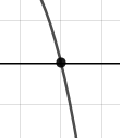
\includegraphics[width = 0.3\textwidth]{../Figures/polyZeroBehaviorCopyAB.png}\item 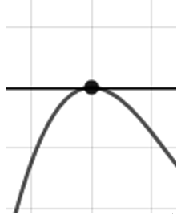
\includegraphics[width = 0.3\textwidth]{../Figures/polyZeroBehaviorCopyBB.png}\item 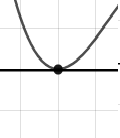
\includegraphics[width = 0.3\textwidth]{../Figures/polyZeroBehaviorCopyCB.png}\item 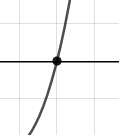
\includegraphics[width = 0.3\textwidth]{../Figures/polyZeroBehaviorCopyDB.png}\end{multicols}\item None of the above.
\end{enumerate} }
\litem{
Which of the following equations \textit{could} be of the graph presented below?
\begin{center}
    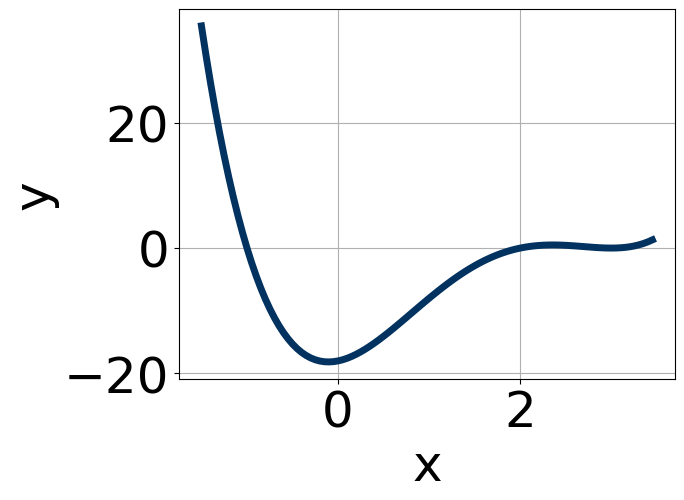
\includegraphics[width=0.5\textwidth]{../Figures/polyGraphToFunctionCopyB.png}
\end{center}
\begin{enumerate}[label=\Alph*.]
\item \( 18(x - 3)^{4} (x - 2)^{10} (x + 1)^{11} \)
\item \( 5(x - 3)^{10} (x - 2)^{11} (x + 1)^{11} \)
\item \( -14(x - 3)^{10} (x - 2)^{11} (x + 1)^{4} \)
\item \( 18(x - 3)^{7} (x - 2)^{4} (x + 1)^{7} \)
\item \( -10(x - 3)^{4} (x - 2)^{9} (x + 1)^{11} \)

\end{enumerate} }
\litem{
Construct the lowest-degree polynomial given the zeros below. Then, choose the intervals that contain the coefficients of the polynomial in the form $x^3+bx^2+cx+d$.\[ -3 - 4 i \text{ and } -3 \]\begin{enumerate}[label=\Alph*.]
\item \( b \in [-3, 3], c \in [6.2, 9.3], \text{ and } d \in [12, 14] \)
\item \( b \in [-12, -8], c \in [42, 47.2], \text{ and } d \in [-75, -74] \)
\item \( b \in [9, 13], c \in [42, 47.2], \text{ and } d \in [72, 82] \)
\item \( b \in [-3, 3], c \in [2.5, 6.7], \text{ and } d \in [5, 11] \)
\item \( \text{None of the above.} \)

\end{enumerate} }
\litem{
Which of the following equations \textit{could} be of the graph presented below?
\begin{center}
    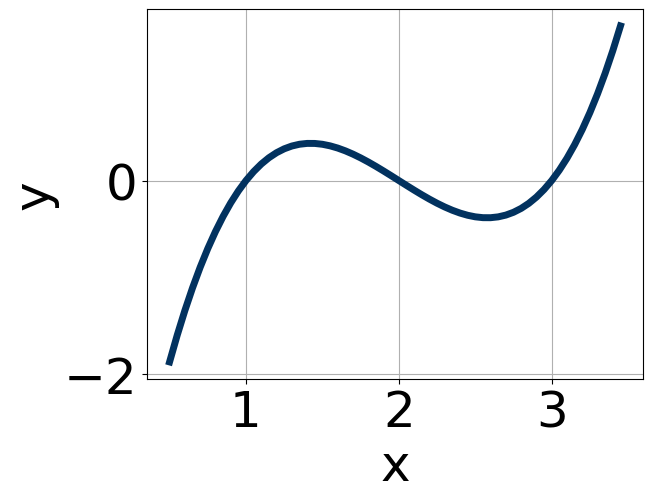
\includegraphics[width=0.5\textwidth]{../Figures/polyGraphToFunctionB.png}
\end{center}
\begin{enumerate}[label=\Alph*.]
\item \( -20(x - 1)^{8} (x - 2)^{9} (x - 3)^{5} \)
\item \( 20(x - 1)^{8} (x - 2)^{5} (x - 3)^{7} \)
\item \( -5(x - 1)^{11} (x - 2)^{11} (x - 3)^{5} \)
\item \( 4(x - 1)^{7} (x - 2)^{5} (x - 3)^{9} \)
\item \( 7(x - 1)^{8} (x - 2)^{6} (x - 3)^{7} \)

\end{enumerate} }
\litem{
Describe the zero behavior of the zero $x = 5$ of the polynomial below.\[ f(x) = 4(x - 2)^{6}(x + 2)^{3}(x - 5)^{7}(x + 5)^{2} \]\begin{enumerate}[label=\Alph*.]
\begin{multicols}{2}\item 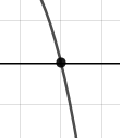
\includegraphics[width = 0.3\textwidth]{../Figures/polyZeroBehaviorAB.png}\item 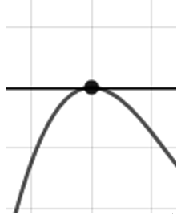
\includegraphics[width = 0.3\textwidth]{../Figures/polyZeroBehaviorBB.png}\item 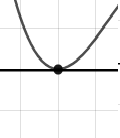
\includegraphics[width = 0.3\textwidth]{../Figures/polyZeroBehaviorCB.png}\item 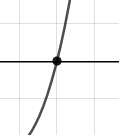
\includegraphics[width = 0.3\textwidth]{../Figures/polyZeroBehaviorDB.png}\end{multicols}\item None of the above.
\end{enumerate} }
\litem{
Describe the end behavior of the polynomial below.\[ f(x) = -2(x + 2)^{3}(x - 2)^{8}(x - 9)^{4}(x + 9)^{6} \]\begin{enumerate}[label=\Alph*.]
\begin{multicols}{2}\item 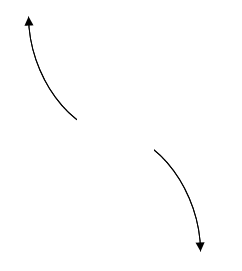
\includegraphics[width = 0.3\textwidth]{../Figures/polyEndBehaviorAB.png}\item 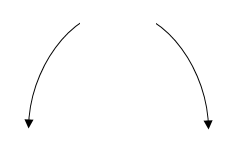
\includegraphics[width = 0.3\textwidth]{../Figures/polyEndBehaviorBB.png}\item 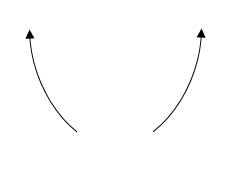
\includegraphics[width = 0.3\textwidth]{../Figures/polyEndBehaviorCB.png}\item 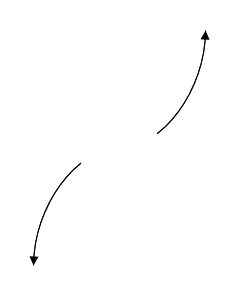
\includegraphics[width = 0.3\textwidth]{../Figures/polyEndBehaviorDB.png}\end{multicols}\item None of the above.
\end{enumerate} }
\litem{
Describe the end behavior of the polynomial below.\[ f(x) = -4(x - 5)^{5}(x + 5)^{8}(x - 4)^{5}(x + 4)^{5} \]\begin{enumerate}[label=\Alph*.]
\begin{multicols}{2}\item 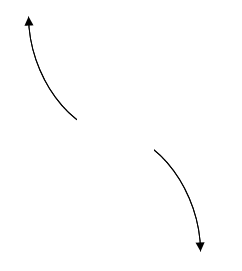
\includegraphics[width = 0.3\textwidth]{../Figures/polyEndBehaviorCopyAB.png}\item 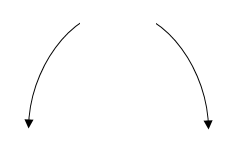
\includegraphics[width = 0.3\textwidth]{../Figures/polyEndBehaviorCopyBB.png}\item 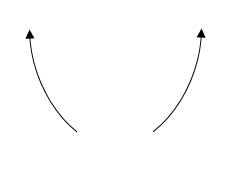
\includegraphics[width = 0.3\textwidth]{../Figures/polyEndBehaviorCopyCB.png}\item 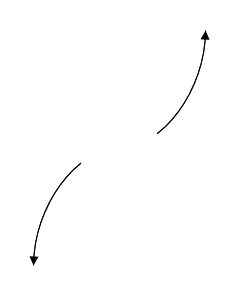
\includegraphics[width = 0.3\textwidth]{../Figures/polyEndBehaviorCopyDB.png}\end{multicols}\item None of the above.
\end{enumerate} }
\litem{
Construct the lowest-degree polynomial given the zeros below. Then, choose the intervals that contain the coefficients of the polynomial in the form $ax^3+bx^2+cx+d$.\[ \frac{4}{3}, \frac{1}{4}, \text{ and } 1 \]\begin{enumerate}[label=\Alph*.]
\item \( a \in [11, 21], b \in [-0.6, 2.1], c \in [-19.5, -16.4], \text{ and } d \in [2, 6] \)
\item \( a \in [11, 21], b \in [1.5, 8.2], c \in [-16, -14.6], \text{ and } d \in [-6, 0] \)
\item \( a \in [11, 21], b \in [30.9, 32.5], c \in [20.5, 27.3], \text{ and } d \in [2, 6] \)
\item \( a \in [11, 21], b \in [-32.9, -28.5], c \in [20.5, 27.3], \text{ and } d \in [-6, 0] \)
\item \( a \in [11, 21], b \in [-32.9, -28.5], c \in [20.5, 27.3], \text{ and } d \in [2, 6] \)

\end{enumerate} }
\litem{
Construct the lowest-degree polynomial given the zeros below. Then, choose the intervals that contain the coefficients of the polynomial in the form $x^3+bx^2+cx+d$.\[ -2 + 3 i \text{ and } -1 \]\begin{enumerate}[label=\Alph*.]
\item \( b \in [0.1, 3.9], c \in [-7, 0], \text{ and } d \in [-5.5, -1.1] \)
\item \( b \in [-10.8, -3], c \in [12, 26], \text{ and } d \in [-14.5, -9.4] \)
\item \( b \in [0.1, 3.9], c \in [2, 8], \text{ and } d \in [0.4, 3.8] \)
\item \( b \in [2.5, 6.7], c \in [12, 26], \text{ and } d \in [12.3, 16.1] \)
\item \( \text{None of the above.} \)

\end{enumerate} }
\litem{
Construct the lowest-degree polynomial given the zeros below. Then, choose the intervals that contain the coefficients of the polynomial in the form $ax^3+bx^2+cx+d$.\[ \frac{7}{4}, \frac{-7}{5}, \text{ and } \frac{5}{2} \]\begin{enumerate}[label=\Alph*.]
\item \( a \in [39, 49], b \in [114, 119], c \in [-65, -62], \text{ and } d \in [-247, -238] \)
\item \( a \in [39, 49], b \in [-87, -83], c \in [-137, -129], \text{ and } d \in [241, 248] \)
\item \( a \in [39, 49], b \in [-115, -112], c \in [-65, -62], \text{ and } d \in [241, 248] \)
\item \( a \in [39, 49], b \in [-115, -112], c \in [-65, -62], \text{ and } d \in [-247, -238] \)
\item \( a \in [39, 49], b \in [25, 29], c \in [-220, -214], \text{ and } d \in [-247, -238] \)

\end{enumerate} }
\litem{
Describe the zero behavior of the zero $x = -8$ of the polynomial below.\[ f(x) = 3(x + 7)^{11}(x - 7)^{9}(x - 8)^{8}(x + 8)^{5} \]\begin{enumerate}[label=\Alph*.]
\begin{multicols}{2}\item 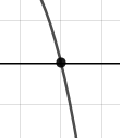
\includegraphics[width = 0.3\textwidth]{../Figures/polyZeroBehaviorCopyAC.png}\item 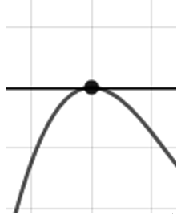
\includegraphics[width = 0.3\textwidth]{../Figures/polyZeroBehaviorCopyBC.png}\item 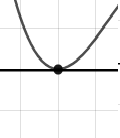
\includegraphics[width = 0.3\textwidth]{../Figures/polyZeroBehaviorCopyCC.png}\item 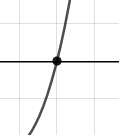
\includegraphics[width = 0.3\textwidth]{../Figures/polyZeroBehaviorCopyDC.png}\end{multicols}\item None of the above.
\end{enumerate} }
\litem{
Which of the following equations \textit{could} be of the graph presented below?
\begin{center}
    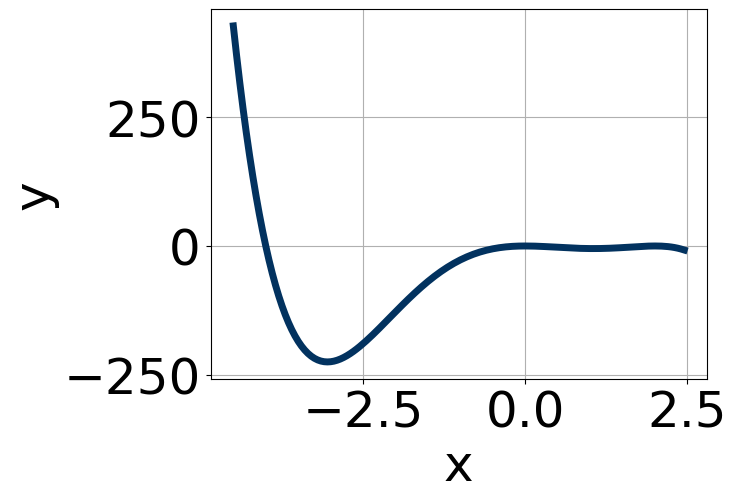
\includegraphics[width=0.5\textwidth]{../Figures/polyGraphToFunctionCopyC.png}
\end{center}
\begin{enumerate}[label=\Alph*.]
\item \( -20x^{4} (x - 2)^{8} (x + 4)^{11} \)
\item \( -4x^{8} (x - 2)^{11} (x + 4)^{7} \)
\item \( 6x^{4} (x - 2)^{6} (x + 4)^{8} \)
\item \( -7x^{8} (x - 2)^{5} (x + 4)^{8} \)
\item \( 14x^{6} (x - 2)^{10} (x + 4)^{7} \)

\end{enumerate} }
\litem{
Construct the lowest-degree polynomial given the zeros below. Then, choose the intervals that contain the coefficients of the polynomial in the form $x^3+bx^2+cx+d$.\[ -5 - 3 i \text{ and } -2 \]\begin{enumerate}[label=\Alph*.]
\item \( b \in [-1, 10], c \in [6.99, 8.99], \text{ and } d \in [7, 12] \)
\item \( b \in [-16, -10], c \in [53.47, 55.02], \text{ and } d \in [-72, -63] \)
\item \( b \in [-1, 10], c \in [4.6, 5.04], \text{ and } d \in [1, 7] \)
\item \( b \in [11, 13], c \in [53.47, 55.02], \text{ and } d \in [68, 69] \)
\item \( \text{None of the above.} \)

\end{enumerate} }
\litem{
Which of the following equations \textit{could} be of the graph presented below?
\begin{center}
    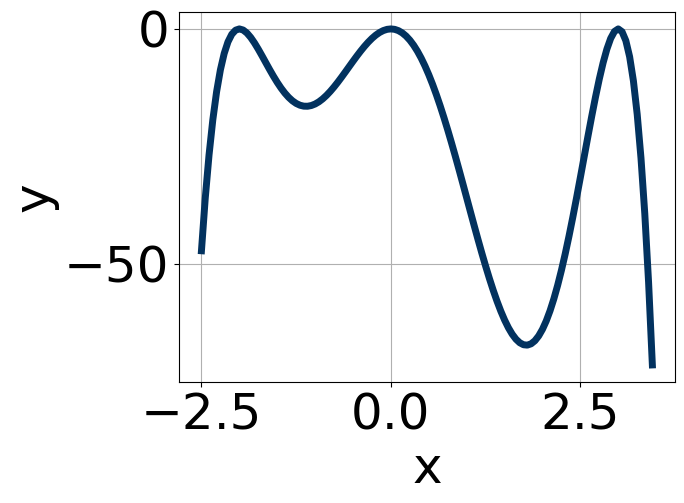
\includegraphics[width=0.5\textwidth]{../Figures/polyGraphToFunctionC.png}
\end{center}
\begin{enumerate}[label=\Alph*.]
\item \( -13x^{10} (x - 3)^{4} (x + 2)^{11} \)
\item \( 11x^{4} (x - 3)^{4} (x + 2)^{4} \)
\item \( -17x^{4} (x - 3)^{10} (x + 2)^{4} \)
\item \( -8x^{8} (x - 3)^{7} (x + 2)^{7} \)
\item \( 12x^{10} (x - 3)^{10} (x + 2)^{11} \)

\end{enumerate} }
\litem{
Describe the zero behavior of the zero $x = 3$ of the polynomial below.\[ f(x) = 5(x - 3)^{5}(x + 3)^{10}(x + 9)^{6}(x - 9)^{10} \]\begin{enumerate}[label=\Alph*.]
\begin{multicols}{2}\item 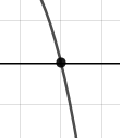
\includegraphics[width = 0.3\textwidth]{../Figures/polyZeroBehaviorAC.png}\item 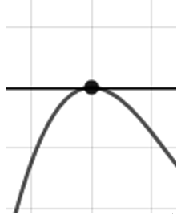
\includegraphics[width = 0.3\textwidth]{../Figures/polyZeroBehaviorBC.png}\item 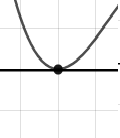
\includegraphics[width = 0.3\textwidth]{../Figures/polyZeroBehaviorCC.png}\item 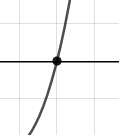
\includegraphics[width = 0.3\textwidth]{../Figures/polyZeroBehaviorDC.png}\end{multicols}\item None of the above.
\end{enumerate} }
\litem{
Describe the end behavior of the polynomial below.\[ f(x) = 2(x + 7)^{3}(x - 7)^{8}(x - 2)^{2}(x + 2)^{4} \]\begin{enumerate}[label=\Alph*.]
\begin{multicols}{2}\item 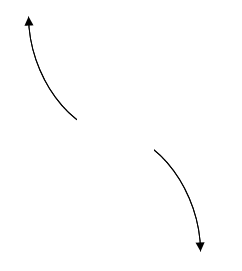
\includegraphics[width = 0.3\textwidth]{../Figures/polyEndBehaviorAC.png}\item 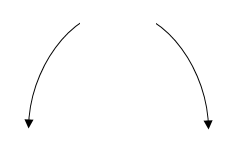
\includegraphics[width = 0.3\textwidth]{../Figures/polyEndBehaviorBC.png}\item 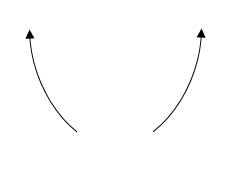
\includegraphics[width = 0.3\textwidth]{../Figures/polyEndBehaviorCC.png}\item 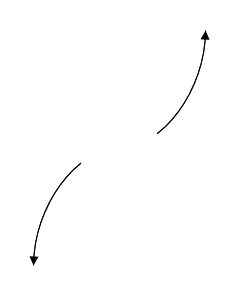
\includegraphics[width = 0.3\textwidth]{../Figures/polyEndBehaviorDC.png}\end{multicols}\item None of the above.
\end{enumerate} }
\litem{
Describe the end behavior of the polynomial below.\[ f(x) = -8(x - 9)^{4}(x + 9)^{5}(x + 2)^{4}(x - 2)^{5} \]\begin{enumerate}[label=\Alph*.]
\begin{multicols}{2}\item \includegraphics[width = 0.3\textwidth]{../Figures/polyEndBehaviorCopyAC.png}\item \includegraphics[width = 0.3\textwidth]{../Figures/polyEndBehaviorCopyBC.png}\item \includegraphics[width = 0.3\textwidth]{../Figures/polyEndBehaviorCopyCC.png}\item \includegraphics[width = 0.3\textwidth]{../Figures/polyEndBehaviorCopyDC.png}\end{multicols}\item None of the above.
\end{enumerate} }
\litem{
Construct the lowest-degree polynomial given the zeros below. Then, choose the intervals that contain the coefficients of the polynomial in the form $ax^3+bx^2+cx+d$.\[ \frac{-1}{4}, \frac{-1}{5}, \text{ and } \frac{4}{5} \]\begin{enumerate}[label=\Alph*.]
\item \( a \in [97, 105], b \in [-39, -33], c \in [-38, -27], \text{ and } d \in [2, 6] \)
\item \( a \in [97, 105], b \in [-125, -121], c \in [36, 47], \text{ and } d \in [-7, -2] \)
\item \( a \in [97, 105], b \in [-87, -79], c \in [-1, 8], \text{ and } d \in [2, 6] \)
\item \( a \in [97, 105], b \in [-39, -33], c \in [-38, -27], \text{ and } d \in [-7, -2] \)
\item \( a \in [97, 105], b \in [32, 40], c \in [-38, -27], \text{ and } d \in [2, 6] \)

\end{enumerate} }
\litem{
Construct the lowest-degree polynomial given the zeros below. Then, choose the intervals that contain the coefficients of the polynomial in the form $x^3+bx^2+cx+d$.\[ 3 - 3 i \text{ and } 4 \]\begin{enumerate}[label=\Alph*.]
\item \( b \in [-1, 7], c \in [-6, 0], \text{ and } d \in [-14, -11] \)
\item \( b \in [-1, 7], c \in [-8, -2], \text{ and } d \in [10, 13] \)
\item \( b \in [5, 20], c \in [34, 44], \text{ and } d \in [72, 78] \)
\item \( b \in [-10, -5], c \in [34, 44], \text{ and } d \in [-77, -69] \)
\item \( \text{None of the above.} \)

\end{enumerate} }
\end{enumerate}

\end{document}